\section{3D scene representation: State of the art approaches}
\label{section:3d scene representation}

% The purpose of this chapter is to gives an overview of different approaches of 3D reconstruction with RGB-D cameras. It presents also telepresence.

A lot have been done in the literature to represent 3D data. This purpose of this section is not to do a survey of it but to present some of the most relevant references and survey paper for further read. It also explains why the point cloud approach is chosen.


\subsection{3D reconstruction with RGB-D cameras}

A state of the art of 3D reconstruction with RGB-D cameras is proposed by \cite{zollhofer_state_2018}. This reference gives a good overview of the actual technology. It makes a distinction between static and dynamic scenes. As people in a meeting room are moving, dynamic approaches are the one that are interesting. This subsection will focus, therefore, on non-rigid reconstruction of dynamic scenes. The 3D representation in the following presented methods is structured meshes.

\subsubsection{Strong scene priors}

Some approaches use strong prior of the scene to simplify the reconstruction. The first real-time template based tracking approach was proposed by \cite{zollhofer_real-time_2014}. A template has to be acquired before any application. Then the live data is fitted to the acquired template to make it move. The demonstration was done for faces and upper body sequences. This kind of approaches gives realistic result, in general. However, it is not suitable for the targeting scenario at Logitech. Scanning people before attending a discussion in a meeting room is not realistic.

\subsubsection{Template-free deformable reconstruction}

Reconstruction of a dynamic scene without any template is a more challenging problem. The first approach to tackle it is called \textit{DynamicFusion} \cite{zollhofer_real-time_2014}. This method progressively reconstructs a moving scene. It updates a model frame after frame in real time. The quality and the details of the reconstruction improves over time. Despite a nice rendering it is not appropriate for the target application. It needs about 30 seconds to have a good reconstruction and the rendering doesn't have colours. 

\textit{Fusion4D} \cite{dou_fusion4d:_2016} which is the basis of \textit{Holoportation} \cite{orts-escolano_holoportation_2016} and \textit{Montage4D} \cite{du_montage4d:_2019}, allows for topological changes in the scene by periodic resets of the reference model. The result is impressive but requires a complex multi-view set-up of 8 specific pots. Each one is composed of 2 infrared and 1 colour camera. The complexity of this approach makes it not really applicable for the meeting room scenario.


\subsection{Telepresence}

According to the defintion of Wikipedia\footnote{Telepresence: \url{https://en.wikipedia.org/wiki/Telepresence}. Last visit: the 22nd of January}: "Telepresence refers to a set of technologies which allow a person to feel as if they were present, to give the appearance of being present, or to have an effect, via telerobotics, at a place other than their true location". This is relevant for a meeting room scenario. A state of the art in telepresence is proposed in \cite{smolic_state---art_nodate}. It presents different capture set-ups and develops a comparison between mesh and point cloud. These are the two main techniques for visualising 3D data.

Mesh means using series of connected faces/polygon to approximate the surface of the original object being represented. Increasing the polygon densities improves the realism of the rendering, see figure \ref{figure:bunny_mesh}.

\begin{figure}[H]
    \centering
    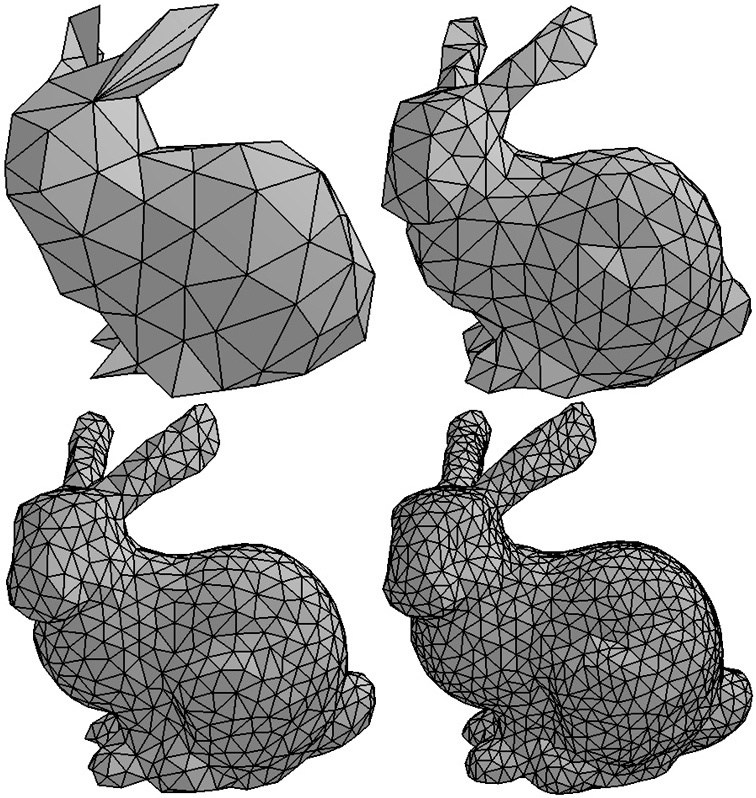
\includegraphics[width=0.35\textwidth]{images/state_of_the_art/bunny_mesh.jpg}
    \caption{Rendering of the Stanford bunny with different mesh densities. Source \cite{smolic_state---art_nodate}}
    \label{figure:bunny_mesh}
\end{figure}

 Despite computational efficiency, \cite{smolic_state---art_nodate} argues that polygon meshes start to become too complex to handle when the level of detail for describing a mesh increases. In such a case, point clouds have to be considered. In point clouds, surfaces are represented as a cloud. An advantage of point clouds over mesh is the fact that dense point clouds can be acquired easily directly with the actual technology. Therefore, this point cloud approach is the one chosen in this master thesis. \textit{LiveScan3D} \cite{kowalski_livescan3d:_2015} proposes a 3D acquisition system for multiple Kinect v2 cameras. Point clouds are used for the rendering of the scene. \textit{LiveScan3D} proposes a calibration step based on markers with a refinement step based on Iterative Closest Point (ICP). This kind of approach will be tested in the chapter \ref{section:Registration} but won't be chosen. \textit{LiveScan3D} raises some issues like colour inconsistency and mis-coloured edges. They are not handled by them. This master thesis will propose some approaches to tackle these kind of problems.